\chapter{Technologien zur Erstellung von 3D Computergrafiken}
\label{chap_technologien}
Dieses Kapitel bietet einen Überblick über die Technologielandschaft zur Erstellung von 3D Computergrafiken. Konkret wird auf populäre Spiele Engines wie Unity, Godot sowie Unreal Engine eingegangen. Nebst den Engines werden auch verschiedene Frameworks wie Three.js sowie Babylon.js thematisiert. Abschliessend wird auf immersive Technologien wie \acrshort{VR} sowie \acrshort{CAVE} eingegangen.

\section{Engines}
Engines sind umfassende Programme, welche das Erstellen von 3D Computergrafiken und insbesondere Videospielen für jedermann zugänglich machen. Anders als Frameworks beinhalten diese Programme integrierte Editoren, welche das Erstellen von 3D-Welten und interaktiven Erlebnissen vereinfachen. Für komplexe Elemente wie Physik- und Audiosysteme werden fertige Komponenten zur Verfügung gestellt. Auch im Bereich der Spiele Engines existieren sowohl kostenlose als auch kostenpflichtige Varianten. Nachfolgend werden die populärsten 3D-fokussierten Engines aus beiden Bereichen vorgestellt. 

\subsection{Unity Engine}
Rückblickend auf das Jahr 2024 bezogen ist die Unity Engine die meistgenutzte Spiele Engine für kleinere bis mittelgrosse 3D Erlebnisse (siehe Abbildung \ref{fig_nutzung_spiele_engines}). Unity gehört zu den kostenpflichtigen Spiele Engines und unterstützt rund 20 verschiedene Plattformen. Angefangen bei den klassischen Desktop-Betriebssystemen wie MacOS, Linux und Windows über Webbrowser bis zu verschiedenen Spielekonsolen und VR-Headsets \parencite{unity_platform_support_2025}.
\begin{figure}[H]
    \caption{Übersicht Nutzung Spiele Engine nach Spielgrösse \parencite[S. 7]{vgi_report_2025}}
    \includegraphics[width=.5\linewidth]{content/00_assets/uebersicht_nutzung_spielengines.png}
    \label{fig_nutzung_spiele_engines}
\end{figure}

Die Spiele selbst werden in Unity innerhalb des Unity-Editors (siehe Abbildung \ref{fig_unity_editor}) und mithilfe der Programmiersprache C-Sharp entwickelt. 
\begin{figure}[H]
    \caption{Unity Editor \parencite{unity_editor_2019}}
    \includegraphics[width=.5\linewidth]{content/00_assets/unity_editor.jpg}
    \label{fig_unity_editor}
\end{figure}

Für Unity existieren verschiedene Lizenzmodelle. Das Lizenzmodell ist hierbei nicht nur vom Funktionsumfang, sondern auch vom Jahreseinkommen abhängig (siehe Tabelle \ref{table_unity_preise}). Für das Erstellen von industriellen Anwendungen muss zudem eine spezielle ``Industry-Lizenz'' erworben werden (Preis auf Anfrage).
\begin{table}[H]
    \caption{Lizenzkosten der Unity Engine in Abhängigkeit zum Jahreseinkommen \parencite{unity_preise_2025}}
    \begin{tabularx}{\textwidth} {
        >{\raggedright\arraybackslash}X 
        >{\raggedright\arraybackslash}X
        >{\raggedright\arraybackslash}X}
            \hline
            \textbf{Lizenzmodell} & {Jahreseinkommen} & {Jahreskosten}  \\
            \hline
            Personal & weniger als 200'000 USD & {Gratis}\\
            Pro & zwischen 200'000 USD und 25'000'000 USD & 2'220 USD pro Nutzer \\
            Enterprise & mehr als 25'000'000 USD &  auf Anfrage \\
            \hline
    \end{tabularx}
    \bigbreak
    \label{table_unity_preise}
\end{table}

\subsection{Unreal Engine}
Über die Jahre haben viele Spielentwicklungsstudios veröffentlicht, dass sie ihre eigens entwickelte Engine durch die Unreal Engine ersetzen werden \parencite[S. 11]{vgi_report_2025}. Unreal Engine zeichnet sich durch die beeindruckenden visuellen Effekte aus. Sie wird jedoch nicht nur zur Entwicklung von Videospielen eingesetzt, sondern kommt auch im Rahmen von Filmproduktionen sowie Architekturvisualisierungen (siehe Abbildung \ref{fig_unreal_engine_architektur}) zum Einsatz. Insbesondere im Architekturbereich werden hierbei gängige Datenformate wie \acrfull{BIM} \parencite{unreal_engine_architektur_2025} unterstützt.
\begin{figure}[H]
    \caption{Unreal Engine Achitektur Visualisierung \parencite{unreal_engine_architektur_2025}}
    \includegraphics[width=.5\linewidth]{content/00_assets/unreal_engine_achitektur.png}
    \label{fig_unreal_engine_architektur}
\end{figure}

Auch die Unreal Engine zählt zu den kommerziellen Spiele Engines, wobei beim Lizenzmodell zwischen zwei verschiedenen Kategorien unterschieden wird. Werden Videospiele erstellt, so ist eine kostenlose Nutzung bis zu einem Umsatz von einer Million USD möglich. Danach werden 5\% des Gewinns als Lizenzgebühren fällig. Werden hingegen Produkte abseits von Videospielen entwickelt, so fallen nach der ersten Million rund 1'800 USD an jährlichen Lizenzgebühren an \parencite{unreal_engine_lizenzkosten_2025}. 

Nebst einem integrierten Editor werden von Unreal Engine zahlreiche Tools für die Erstellung von immersiven Erlebnissen angeboten. Mithilfe des World Partitioning Tools können riesige 3D-Welten erstellt werden. Hierbei wird die virtuelle Welt anhand eines Gitternetzes in dedizierte Teilbereiche unterteilt. Während sich Personen durch die Welt bewegen, werden diese Bereiche dynamisch geladen \parencite{unreal_engine_2025}. Auch bei der Erstellung von 3D Modellen wird Unterstützung geboten. Quixel Megascan ermöglicht die Integration von fotogrammetrisch erzeugten Geometrien sowie die Nutzung von hochauflösenden Texturen \parencite{unreal_engine_quixel_2025}. Die eigentliche Logik der 3D Visualisierungen wird in Unreal mithilfe der systemnahen Programmiersprache C++ sowie einer visuellen Scriptsprache namens ``Blueprints'' umgesetzt. Blueprints erlaubt es, komplexe Funktionalitäten mithilfe eines Node-Systems umzusetzen (siehe Abbildung \ref{fig_unreal_engine_blueprints}). Dadurch können auch Personen ohne vertiefe Programmierkenntnisse unterschiedliche Konzepte erproben, während komplexe Aspekte in C++ implementiert werden. 
\begin{figure}[H]
    \caption{Unreal Engine Blueprints \parencite{unreal_engine_blueprints_2026}}
    \includegraphics[width=.5\linewidth]{content/00_assets/unreal_engine_blueprints.png}
    \label{fig_unreal_engine_blueprints}
\end{figure}

\subsection{Godot Engine}
Nebst kommerziellen Engines wie Unity und Unreal gibt es auch kostenlose Alternativen wie die Godot Engine. Die Engine basiert auf der MIT Open Source Lizenz und bietet uneingeschränkte Nutzungsrechte sowie Zugriff auf den gesamten Quellcode \parencite{godot_mit_license_2023}.  
Godot benötigt im Vergleich zu Unity und Unreal Engine auch signifikant weniger Speicherplatz. Für die Engine werden lediglich zwischen 200MB und 1.5GB Festplattenspeicher benötigt. Dies ist eine erhebliche Reduktion im Vergleich zu den 5 - 20GB der Unity sowie den 30 bis 50GB der Unreal Engine. Wie Unity und Unreal unterstützt auch Godot diverse verschiedene Plattformen. Von den bekannten Betriebssystemen wie MacOS, Linux und Windows über Webbrowser bis zu mobilen Endgeräten wird ein breites Spektrum abgedeckt \parencite{godot_faq_2025}. Ebenso verfügt Godot über einen integrierten Editor, welcher die Erstellung von 3D-Welten erleichtert. Dank der offenen MIT-Lizenz stehen zudem zahlreiche Erweiterungen zur Verfügung, die auf der Engine selbst aufbauen. Mithilfe von Material Maker können beispielsweise prozedurale Texturen erstellt werden (siehe Abbildung \ref{fig_godot_material_maker}). Mittels der App Xogot kann Godot auch auf Apple-Geräten wie dem iPhone oder iPad genutzt werden \parencite{godot_xogot_2025}.
\begin{figure}[H]
    \caption{Material Maker Tool zur Erzeugung von prozeduralen Texturen \parencite{godot_material_maker_2025}}
    \includegraphics[width=.5\linewidth]{content/00_assets/godot_material_maker.png}
    \label{fig_godot_material_maker}
\end{figure}

\section{Frameworks}
Anders als Engines besitzen Frameworks in der Regel keinen integrierten Editor. Stattdessen werden einzelne Bausteine und Programmiermodule für wichtige Funktionalitäten wie 3D Rendering, Audio und Physik Systeme angeboten. Aufgrund des reduzierten Umfangs in Hinblick auf Funktionalität, Tooling sowie unterstützte Plattformen sind Frameworks auch leichtgewichtiger und ressourcenschonender als komplette Spiele Engines. Jedoch ist auch der Programmierer selbst dafür verantwortlich, die einzelnen Bausteine zu einer Gesamtlösung zu kombinieren. Hierdurch entsteht grosser Handlungsfreiraum in Hinblick auf Softwarearchitektur und Funktionsweise. Hierfür müssen jedoch entsprechende technische Grundlagen vorhanden sein.

\subsection{Three.js}
Mit über 3 Millionen Downloads pro Woche zählt Three.js zu den populärsten webbasierten Frameworks für 3D-Grafiken \parencite{threejs_downloads_2025}. Dieses basiert wie die Godot Engine auf der MIT Open Source Lizenz und kann daher ohne Bedenken und Einschränkungen für Projekte aller Art verwendet werden \parencite{threejs_lizenz_2024}. Anders als Unity, Unreal und Godot ist die primäre Zielplattform von Three.js der Browser. Browserbasierte Anwendungen haben den Vorteil, dass keinerlei Installation der Software notwendig ist und gleichzeitig ein breites Spektrum von Endgeräten abgedeckt werden kann. Hierbei werden vom Framework moderne Browser-Grafikschnittstellen wie WebGL2 sowie WebGPU unterstützt. Diese Grafikschnittstellen erlauben die Umsetzung von detailreichen und performanten 3D-Anwendungen. Three.js abstrahiert und vereinheitlicht auch Unterschiede in der Implementierung der Grafikschnittstellen zwischen den einzelnen Browsern. Dadurch werden Browserinkompatibilitäten von 3D-Anwendungen vermieden. Nebst einer umfangreichen Dokumentation\footnote{\url{https://threejs.org/manual/}} stehen über 150 verschiedene Beispielprojekte\footnote{\url{https://threejs.org/examples/}} zur Verfügung. Auch internationale Unternehmen wie Apple setzten bereits Three.js auf der eigenen Webseite ein, um Produkte wie das iPhone in 3D zu bewerben. Das Framework kann aber auch dazu eingesetzt werden, um komplette interaktive und erlebbare 3D-Welten zu erschaffen, wie das Portfolio von Simon Bruno zeigt (siehe Abbildung \ref{fig_threejs_portfolio_simon_bruno}).
\begin{figure}[H]
    \caption{Interaktives Portfolio von Simon Bruno \parencite{threejs_simon_bruno_portfolio_2025}}
    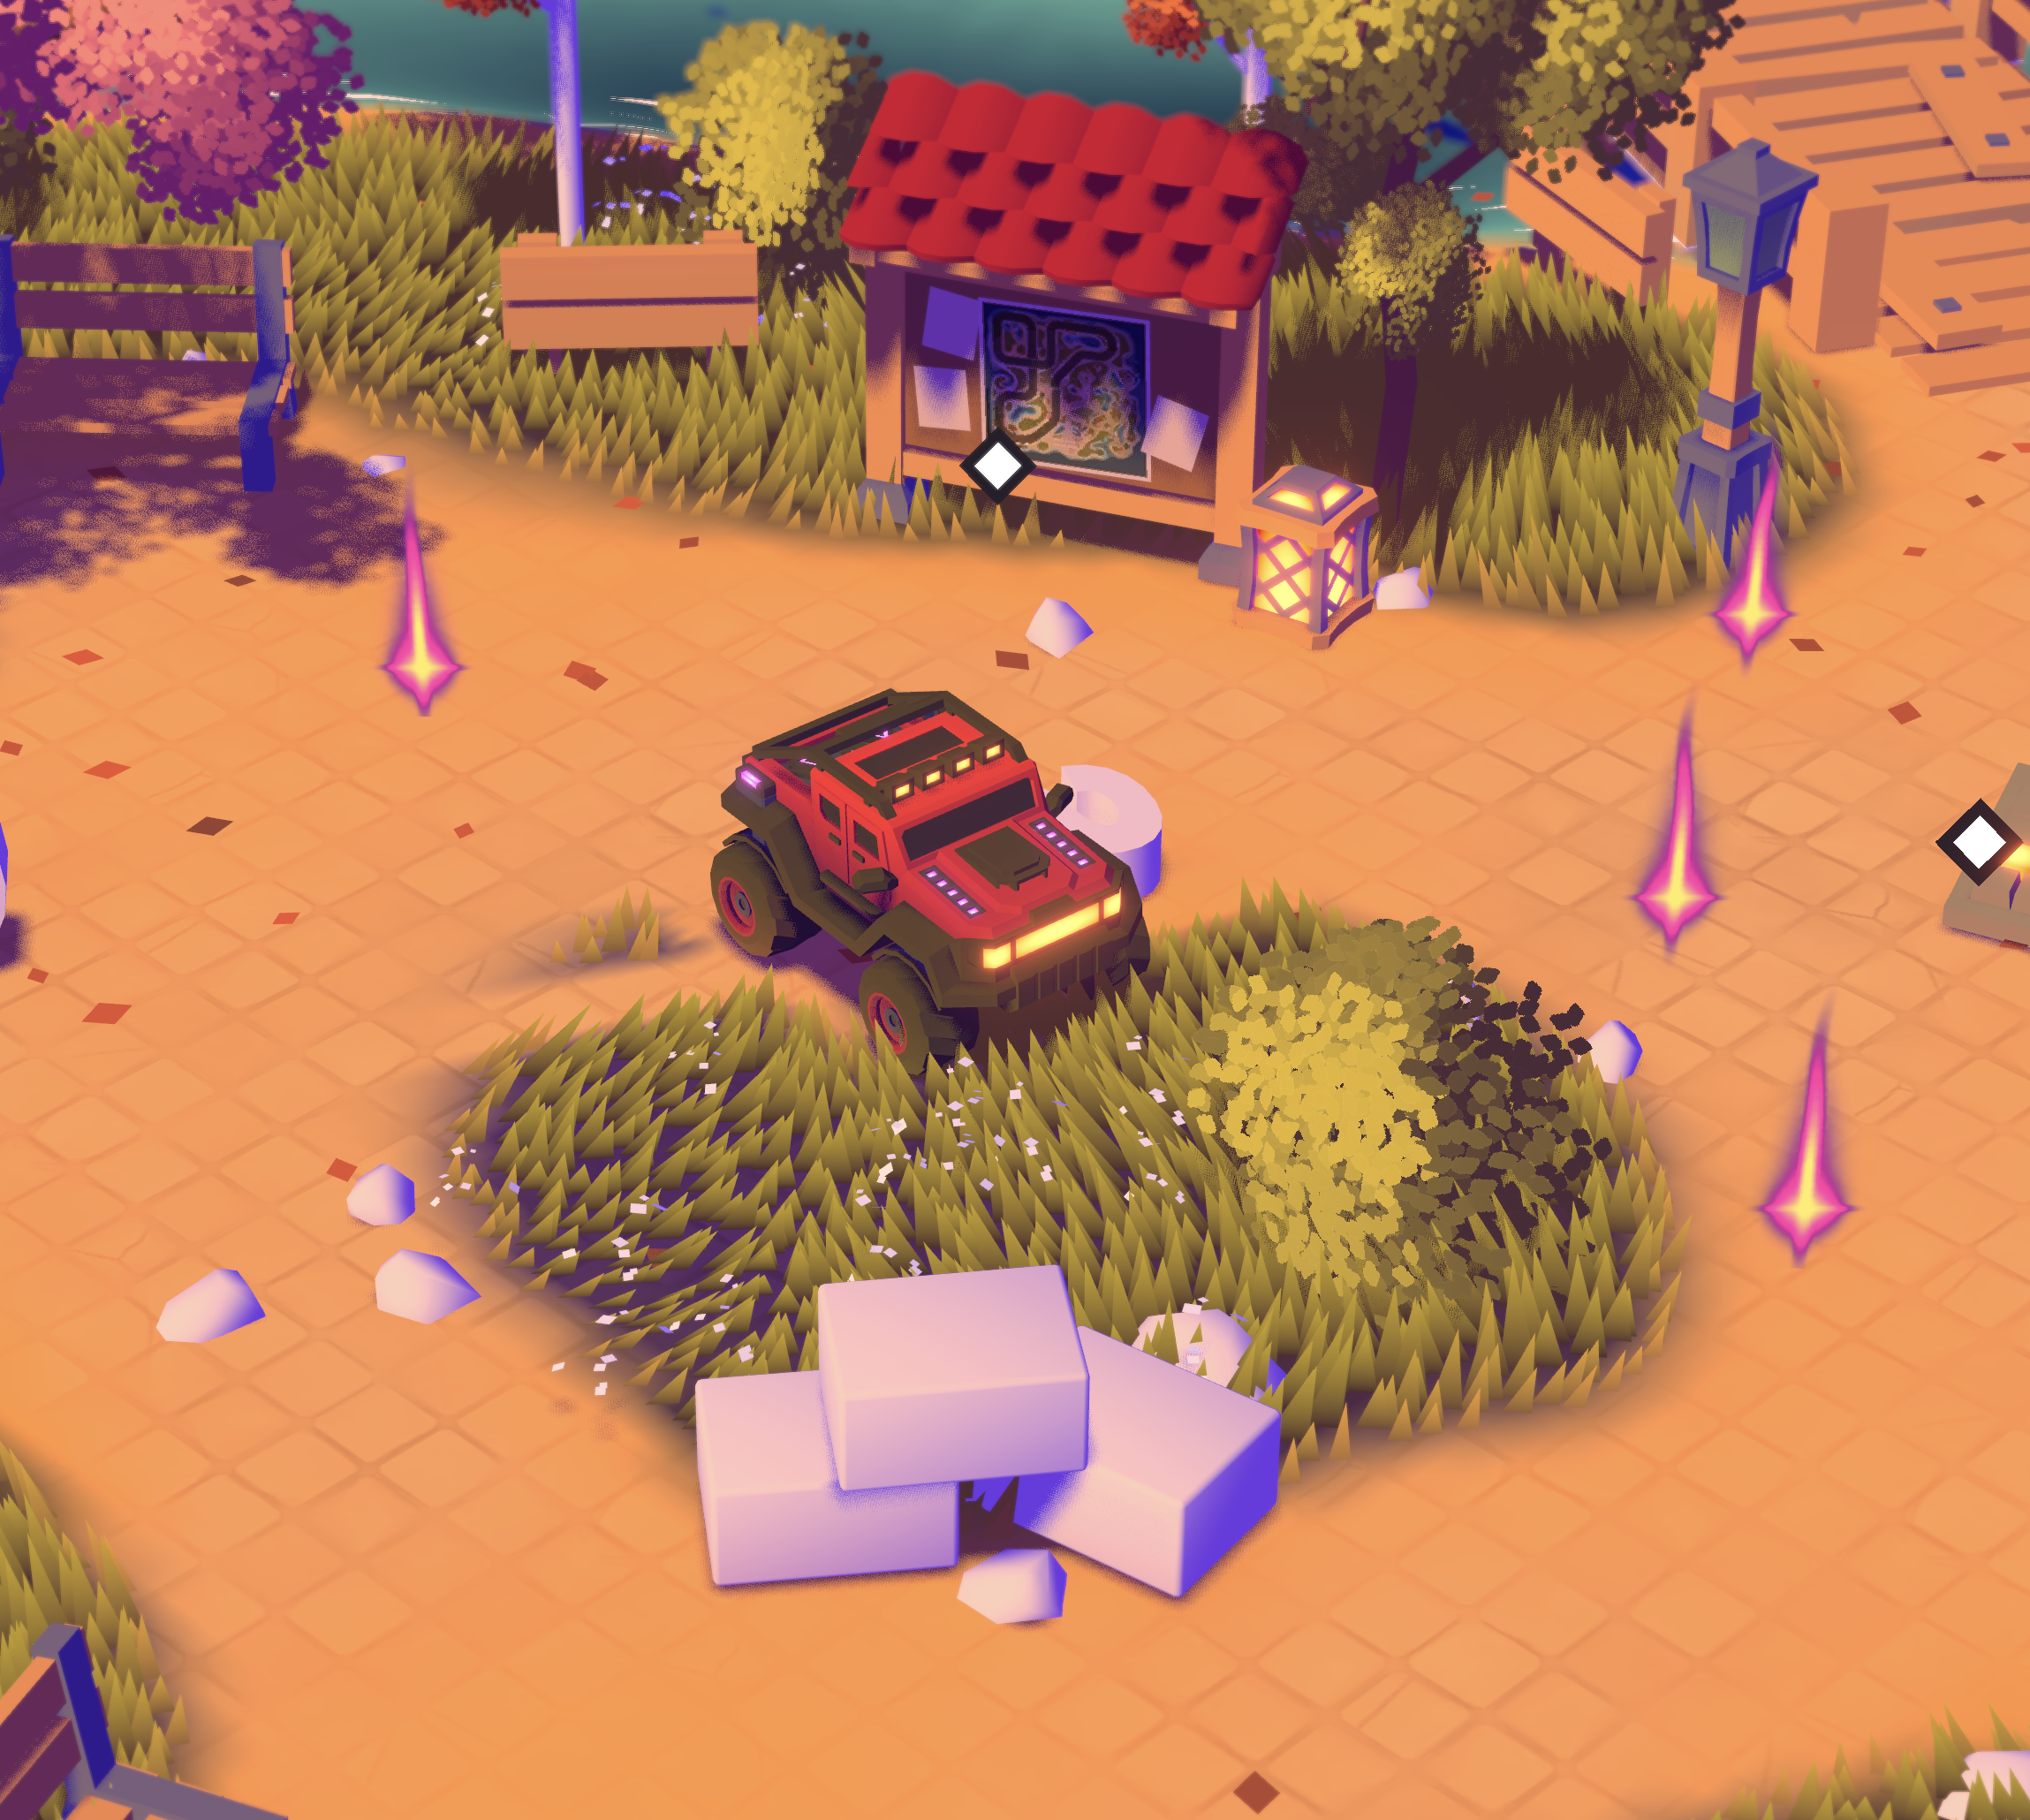
\includegraphics[width=.4\linewidth]{content/00_assets/threejs_portfolio_simon_bruno.png}
    \label{fig_threejs_portfolio_simon_bruno}
\end{figure}

Ebenso können komplette browserbasierte VR-Anwendungen mittels der WebXR-Technologie umgesetzt werden. Die primäre Programmiersprache des Frameworks ist JavaScript. Jedoch können auch Sprachen mit statischer Typisierung wie TypeScript\footnote{\url{https://www.typescriptlang.org}} ohne Probleme verwendet werden. 

\subsection{Babylon.js}
Nebst Three.js ist auch Babylon.js ein sehr prominentes Webframework. Babylon.js wurde im Jahr 2013 von Microsoft basierend auf der Programmiersprache TypeScript entwickelt. Wie Three.js werden sowohl die WebGL2 als auch WebGPU Grafikschnittstelle unterstützt. Im Gegensatz zu Three.js besitzt Babylon.js eine integrierte Physik-Engine, einen Inspektor (siehe Abbildung \ref{fig_babylonjs_inspektor}) sowie einen UI-Editor \parencite{babylonjs_gui_editor_2025}. All diese Features machen Babylon.js zu einem populären Webframework, welches rund 14'600 mal pro Woche heruntergeladen wird \parencite{babylonjs_npm_2025}. Die Downloadgrösse beträgt hierbei rund 60MB und ist somit rund doppelt so gross wie jene von Three.js. Wie Three.js hat auch Babylon.js eine umfassende Dokumentation\footnote{\url{https://doc.babylonjs.com}}. Babylon.js unterscheidet sich jedoch dadurch, dass es im Gegensatz zu dem modularen Ansatz von Three.js in vielen Bereichen eine feste Struktur vorgibt \parencite{babylonjs_vs_threejs_2025}. Aufgrund der Apache 2.0 Open Source Lizenz kann das Framework ohne Bedenken für kommerzielle Zwecke eingesetzt werden \parencite{babylonjs_lizenz_2025}.
\begin{figure}[H]
    \caption{Babylon.js Inspektor \parencite{babylonjs_inspector_2025}}
    \includegraphics[width=.4\linewidth]{content/00_assets/babylonjs_inspektor.png}
    \label{fig_babylonjs_inspektor}
\end{figure}

\subsection{Sokol}
Anders als browserbasierte Anwendungen, laufen native Applikationen direkt auf dem entsprechenden Betriebssystem  und können auch ohne Internetverbindung genutzt werden. Jedes Betriebssystem verwendet hierbei jedoch eine andere Grafikschnittstelle. Unter Windows wird primär DirectX verwendet, wohingegen unter Linux OpenGL sowie Vulkan und bei MacOS die Metal Grafikschnittstelle zum Einsatz kommen. Soll eine Applikation auf allen Betriebssystemen unterstützt werden, muss diese daher für jede Grafikschnittstelle einzeln entwickelt werden. Sokol\footnote{\url{https://github.com/floooh/sokol}} ist ein Framework, welches die verschiedenen Grafikschnittstellen vereinheitlicht. Dies hat den Vorteil, dass die Anwendung nur einmal entwickelt werden muss. Sokol basiert auf der Open Source ZLib Lizenz und kann daher kostenfrei für kommerzielle Projekte eingesetzt werden. Das Framework ist in der systemnahen Programmiersprache C geschrieben und daher besonders performant und speichereffizient. Es stehen diverse Tools zur Verfügung, welche das Arbeiten mit den 3D-Grafikschnittstellen vereinfachen. Mithilfe des ``Shader Code Generator Tool'' \footnote{\url{https://github.com/floooh/sokol-tools/blob/master/docs/sokol-shdc.md}} (sokol-shdc) können Shader für unterschiedliche Grafikschnittstellen generiert werden (eine detailliertere Erklärung zu Shader folgt in Kapitel \ref{chap_render_pipelines}). Nebst den bekannten Betriebssystemen wird auch der Browser als mögliche Zielplattform unterstützt. Hierzu wird \acrfull{Wasm} verwendet, um C-Code in eine für den Browser verständliche Sprache zu übersetzen. \acrshort{Wasm} hat den Vorteil, dass der generierte Code eine geringe Dateigrösse aufweist und effizient ausgeführt wird. Wie Three.js besitzt Sokol einen modularen Aufbau. Die einzelnen Module stehen als sogenannte ``Single Header Library'' zur Verfügung. Das bedeutet, dass sich der gesamte Code in einer einzelnen Datei befindet und keine Abhängigkeiten bestehen. Dies erleichtert die Integration in ein bestehendes Projekt, da jeweils nur eine Datei integriert werden muss und kein komplexes Build-System notwendig ist. Die Dokumentation selbst befindet sich in Form von Quellcode-Kommentaren ebenfalls in den entsprechenden Single Header Libraries. Wie in Three.js bietet auch Sokol diverse Beispiele an, welche auch direkt im Browser angeschaut werden können (siehe Abbildung \ref{fig_sokol_beispiele}).
\begin{figure}[H]
    \caption{Sokol Beispiele \parencite{sokol_beispiele_2025}}
    \includegraphics[width=.6\linewidth]{content/00_assets/sokol_beispiele.png}
    \label{fig_sokol_beispiele}
\end{figure}

\subsection{Electron}
\label{chap_electron}
Es wurden sowohl webbasierte als auch native Frameworks thematisiert. Webbasierte Frameworks haben im Gegensatz zu den nativen Frameworks den Vorteil, dass keine Installation notwendig ist und sie auf einem breiten Spektrum von Endgeräten lauffähig sind. Ein Nachteil von Webframeworks ist jedoch ein sehr eingeschränkter Zugriff auf Dinge wie Multithreading sowie auf das Dateisystem.

Electron\footnote{\url{https://www.electronjs.org}} ist ein Framework, mithilfe dessen browserbasierte Anwendungen direkt auf dem entsprechenden Betriebssystem als native Anwendungen ausgeführt werden können. Electron kombiniert die eigentliche Webanwendung mit einem Chromium Browser sowie einer Node.js-Runtime zu einer nativen Anwendung \parencite{electron_documentation_2025}. Dadurch erhöht sich zwar der Festplattenverbrauch im Vergleich zu einer nativen Anwendung, gleichzeitig erhalten Browseranwendungen jedoch Zugriff auf wichtige systemnahe Funktionalitäten wie Kamera und Dateisystem \parencite{electron_why_2025}. Aufgrund der MIT-Lizenz ist die Nutzung von Electron zudem kostenfrei und uneingeschränkt möglich \parencite{electron_license_2021}.

\subsection{Tauri}
Tauri\footnote{\url{https://v2.tauri.app}} hat wie Electron das Ziel, browserbasierte Anwendungen als native Applikationen auf dem Betriebssystem auszuführen. Anders als Electron verpackt Tauri jedoch nicht einen kompletten Browser in die native Anwendung, sondern benutzt sogenannte ``WebViews''. WebViews sind Softwarekomponenten, welche das Einbinden von browserbasierten Inhalten in nativen Anwendungen erlauben und auf allen gängigen Betriebssystemen vorhanden sind. Anders als vollwertige Browser benötigen WebViews auch um weniger Festplattenspeicher. Eine auf Tauri basierte Anwendung kann somit auf bis zu 600KB reduziert werden. Vergleicht man diesen Wert mit den sonst benötigten 80 - 150MB bei einer Electron Anwendung, ergibt sich hierdurch eine signifikante Ersparnis des Festplattenverbrauches. Unternehmen wie Microsoft verwenden WebViews bereits in eigenen Produkten wie Microsoft Teams \parencite{microsoft_teams_webview_2023}. Um den Zugriff auf native Betriebssystemfunktionalitäten zu ermöglichen, benutzt Tauri verschiedene Module, welche in der systemnahen Programmiersprache Rust geschrieben sind. Ein Nachteil von WebViews, im Gegensatz zu Browsern wie Chromium, besteht darin, dass je nach Betriebssystem Unterschiede in den angebotenen Funktionalitäten auftreten können. Wenn jedoch Festplattenspeicher wie auch eine ressourcenschonendere Anwendung im Vordergrund stehen, ist Tauri eine ansprechende Alternative zu Electron.

\section{Immersive Technologien}
Frameworks und Engines helfen dabei, ansprechende 3D-Erlebnisse zu gestalten. Um jedoch ein immersives Erlebnis zu gewährleisten, reicht dies alleine nicht aus. Technologien wie \acrshort{VR} und \acrshort{CAVE}-Systeme tragen dazu bei, die Immersion für Personen zu erhöhen und ihnen das Gefühl zu vermitteln, sich mitten im virtuellen Erlebnis zu befinden.

\subsection{\acrfull{VR}}
Bei klassischen 3D Anwendungen befinden sich Personen in der Regel vor dem Bildschirm. \acrshort{VR} funktioniert anders. Anstelle eines Bildschirms werden ein \acrshort{VR}-Headset sowie entsprechende Controller verwendet (siehe Abbildung \ref{fig_vr_headset_controller}). Dies sorgt für ein besonders immersives Erlebnis. Mittels Controller können Personen sich durch die virtuelle Welt bewegen, während das Headset eine freie Wahl der Blickrichtung erlaubt. Voraussetzung für ein überzeugendes immersives Erlebnis sind jedoch ausreichender Bewegungsfreiraum sowie eine korrekte Kalibrierung der Geräte. Moderne Browser und Webframeworks wie Three.js und Babylon.js erlauben es, VR-Anwendungen direkt innerhalb des Browsers mithilfe der WebXR\footnote{\url{https://immersiveweb.dev/}}-API umzusetzen. VR-Anwendungen sind somit nicht nur auf native Plattformen und mobile Endgeräte beschränkt und erhalten eine noch breitere Reichweite und Adaption.
\begin{figure}[H]
    \caption{Person mit VR-Headset und Controller \parencite{vr_headset_controller}}
    \includegraphics[width=.3\linewidth]{content/00_assets/vr_headset_controller.jpg}
    \label{fig_vr_headset_controller}
\end{figure}

\subsection{\acrfull{CAVE}}
\label{chap_cave}
Im Gegensatz zu \acrshort{VR} ist bei einem \acrshort{CAVE}-System kein Headset erforderlich. Stattdessen werden ein Raum, in dem sich Personen frei bewegen können, sowie entsprechende Projektoren und Rechner benötigt. Während sich die Personen in der Raummitte befinden, wird die Visualisierung auf die umgebenden Wände projiziert \parencite{cave_1992}. Dadurch entsteht der Eindruck, sich mitten innerhalb der Visualisierung zu befinden. Ein Vorteil von CAVE-Systemen besteht in der einfachen Möglichkeit zur Kollaboration. Mehrere Beteiligte können sich gleichzeitig im selben Raum aufhalten und zentrale Aspekte der Visualisierung gemeinsam diskutieren (siehe Abbildung \ref{fig_cave_collaboration}). Besonders im Bildungsbereich und in wissenschaftlichen Visualisierungen ist dies ein grosser Vorteil \parencite{cave_collaboration_2020}.
\begin{figure}[H]
    \caption{Kollaboration in einem CAVE-System \parencite[S. 11]{cave_collaboration_2020}}
    \includegraphics[width=.5\linewidth]{content/00_assets/cave_collaboration.png}
    \label{fig_cave_collaboration}
\end{figure}

 Die Anschaffungskosten professioneller CAVE-Systeme liegen im Vergleich zu VR-Systemen deutlich höher. Neben dem eigentlichen Raum sind mehrere Projektoren, Rechner sowie weitere Hardware erforderlich. Zusätzlich ist spezialisierte Software notwendig, die eine verzerrungsfreie und synchronisierte Projektion der Visualisierung auf alle Wände ermöglicht. Ein bewährter Ansatz zur Umsetzung dieser Anforderung ist das sogenannte ``Master-Slave'' Konzept \parencite{Flynn2014CAVE}. Pro Wand gibt es einen entsprechenden Rechner und Projektor. Auf jedem Rechner läuft die gleiche Visualisierung. Einer der Rechner (Master) gibt den Takt zur Synchronisierung vor und übermittelt die notwendigen Synchronisationsdaten (Kameraposition etc.) an die anderen Rechner (Slave). Die Slaves visualisieren jeweils ihren eigenen Ausschnitt der Visualisierung in Abhängigkeit von den Synchronisationsdaten und dem vorgegebenen Takt.
 
 Ein CAVE-System kann mit entsprechender Hardware beliebig erweitert werden. Mithilfe von Head Tracking Hardware ist das dynamische Verfolgen der Person im Raum möglich. Hiermit kann sich die Visualisierung dynamisch anhand der Position anpassen und so neue Blickwinkel eröffnen. Aufgrund des breiten Spektrums an Erweiterungsmöglichkeiten ergeben sich auch unterschiedliche Preissegmente, angefangen bei vierstelligen bis zu hohen siebenstelligen Beträgen. Für die Inbetriebnahme der CAVE-Systeme gibt es entsprechend spezialisierte Firmen wie Inside Reality\footnote{\url{https://inside-reality.com/product/icroom}}, welche nebst der entsprechenden Software auch die entsprechende Hardware und Expertise anbieten.